

\documentclass[12pt]{article}
\usepackage[T1]{fontenc}
\usepackage[utf8]{inputenc}
\usepackage{amsmath}
\usepackage{microtype}
\usepackage{listings}
\setlength{\parindent}{0pt}
\usepackage{fancyvrb}
\usepackage{enumerate}
\usepackage{array}
\usepackage[breaklinks=true,linktocpage,hidelinks]{hyperref}
\usepackage[letterpaper]{geometry}
\usepackage{url}
\usepackage{graphicx}
\usepackage{fullpage}

\usepackage{pgfplots}
\usepackage{pgfplotstable}
\usepackage{tikz}

\usepackage{fancyhdr}
\usepackage{fancybox}
\usepackage{multicol}
\usepackage{xcolor}
\usepackage{adjustbox}

\pgfplotsset{compat=newest}
\usetikzlibrary{shapes,backgrounds,arrows}
\usepgfplotslibrary{external} 

\definecolor{brewcol1}{RGB}{166,206,227}
\definecolor{brewcol2}{RGB}{31,120,180}
\definecolor{brewcol3}{RGB}{178,223,138}
\definecolor{brewcol4}{RGB}{51,160,44}
\definecolor{brewcol5}{RGB}{251,154,153}
\definecolor{brewcol6}{RGB}{227,26,28}
\definecolor{brewcol7}{RGB}{237,179,1}
\definecolor{brewcol8}{RGB}{202,178,214}
\definecolor{brewcol9}{RGB}{206,27,1}

\geometry{hmargin=1.87cm, vmargin=1.87cm}
\bibliographystyle{siam}

\DeclareTextFontCommand{\helvetica}{\fontfamily{phv}\selectfont\small}


\begin{document}

\clearpage\thispagestyle{empty}
\begin{center}
\textbf{Difficult transition for sugar maple in Boreal forest under climate change? \\
Impact of alternative stable states on Sugar maple migration.}
\vskip 2em
Research proposal
\vskip 1em
Master in Wildlife management
\vfill
By
\vfill
Steve Vissault 
\vfill 
For
\vfill
\textbf{Richard Cloutier}, Pr.\\
Director of the program committee
\vskip 2em
\textbf{Dominique Arsenault}, Pr.\\
President of the jury
\vskip 2em
\textbf{Matt Talluto}, PhD\\
Research Co-director
\vskip 2em
\textbf{Dominique Gravel}, Pr.\\
Research Director
\vfill
\vfill
Université du Québec à Rimouski\\
\today

\end{center}

\newpage
\setcounter{page}{1}

\section{Introduction.}

\textbf{Context.} The boreal region is warming twice as fast as the global average and will inevitably alter species composition in boreal forest \cite{Scheffer2012,Hughes2000}.  Sugar maple is one of those species expected to migrate northward towards it's nordic temperate forest limits \cite{McKENNEY2007,Goldblum2005}. Predict shifts in the repartition of sugar maple under climate change is an important challenge whereas this species is highly coveted by wood and maple syrup producers, two main economic sectors in Quebec. Indeed, Sugar maple is a widespread and abundant tree in north-eastern North America and one of the most representative species of northern temperate forests \cite{Graignic2013,Messaoud2007,Kellman2004}. This northward migration will result in increasing the surface of the ecotone between the boreal and temperate forest of Quebec. Nevertheless, the expansion of sugar maple distribution could be difficult and explain by the fact than microclimatic conditions found in boreal forests are different from those present in temperate forest. Colder temperatures from shading and excess soil moisture due to snow melt cause litter to be more acidic and fibrous during the spring. Therefore, even if the regional climate conditions are favorable \cite{Kellman2004}, the microbiota conditions found in the boreal forest could affect the establishment of sugar maple \cite{Kellman2004,Moore2008,DeFrenne2013}. In this case, the sugar maple could be unable to migrate in boreal forests as a result of negative soil feedback. This fact could increase the tension between the boreal forest and the nordic temperate forest and generating abrupt changes in the species composition of this ecotone.\\

\textbf{Theorical framework.} Many ecotone studies and modeling efforts on transition between forest to non-forest ecosystems (e. g. Boreal - Toundra) \cite{Scheffer2012,Scheffer2001,Hirota2011} but little attention has been given to evaluate the transitionnal dynamics of forest-forest ecotone \cite{Goldblum2010,Graignic2013}. At regional scale, most transition between differents ecosystems appear often gradually over the time \cite{Scheffer2001,scheffer2009critical}. However, system can \\

\textbf{Natural system.} We used maple sugar basa areal in function of black spruce, white spruce and balsam fir basal area to compute the relative abundance of sugar maple. Given the above statements, we used mainly two climatic variables (annual mean temperature and annual precipitation) to identify the alternative stable states present in the boreal-temperate ecotone. The relationship was performed on climatic variables and sugar maple relative abundance using kernel density plot function. We obtained the probability of observed a sample plot as function of sugar maple relative abundance and mean annual temperature (Figure \ref{fig1}). In both case, alternative stable states are presents whereas the function graphed has a bimodal distribution. At low precipitation or temperature conditions, the probability of observing a parcel sampled without sugar maple is higher than intermediate climatic conditions where the multimodal distribution appear. The density function suggest a double hysterisis of sugar maple states in response of intermediate climatic condition: one state wherein sugar maple dominates and an another in which sugar maple is absent. \\

%% IMPORTANT:: Structurer les points 

\begin{figure}[ht]
	\begin{center}
	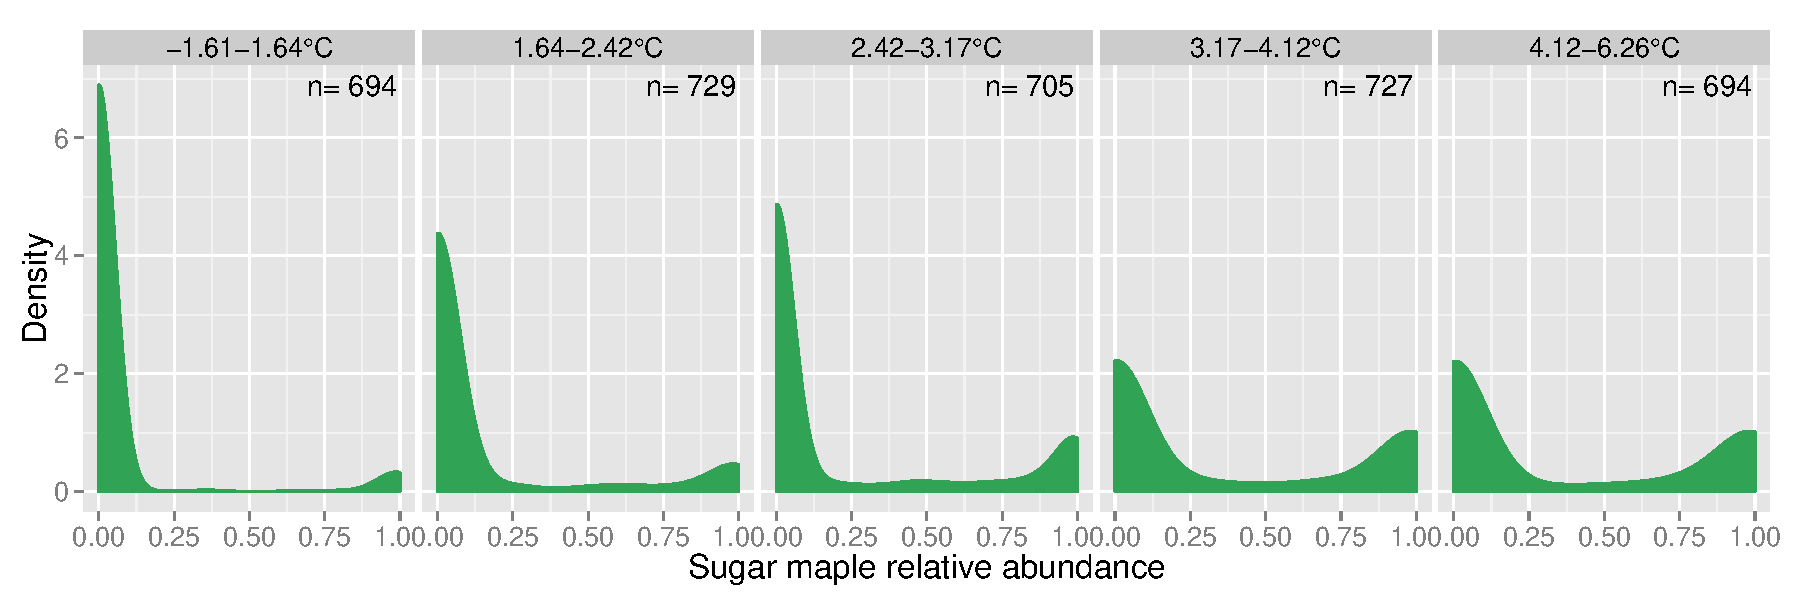
\includegraphics[width=\textwidth]{fig/window_temp.pdf}
	\end{center}
	\caption{Kernel density estimate given the relative abundace of sugar maple. \textbf{Describe the procedure}}
	\label{fig1}
\end{figure}

This project aim to develop a state and transition model (STM) between the boreal and temperate nordic forest in order to investigate the migration rate of sugar maple under different climate change scenarios. To assess this objective, we will use the alternative stable states theory as a framework.

%% Plan
% Theorical framework. 
% Applied this framework to the sugar maple natural system


%(General) finir avec l'objectifs


\section{Objectives.} 

This project aims to determine whether alternative stable states are present in the temperate-boreal forest ecotone and if so, look at the impact of plant-soil and disturbances feedback on the alternatives stables states. To assess this main objective, we will (O1) generate a transitionnal model between the temperate and the boreal forest; (O2) study the equilibrium states based on the model; (O3) investigate the spatial structure of the transitonnal zone; and finaly (O4) run simulations based on different climate change scenarios. \\

\section{Methods.}

\textbf{Models.}

\textbf{Equilibrium study.}

\textbf{Paramerization.} 

\textbf{Validation.}


\newpage
\bibliography{/home/steve/Dropbox/Bibtex/Devis}
\end{document}
